\pagebreak
\section{Introduction}

	The detection of gravitational-waves from  the merger of two black holes in 2015 \citep{GW150914} heralded the onset of a new method of investigating the known universe. Since then there has been a number of other detections of binary black hole coalescences \citep{GW151226, GW170104,GW170814}. Furthermore, a binary neutron star (BNS) merger was detected on 17th August 2017 \citep{GW170817} generating renewed interest in the properties of neutron stars.\par
	
	The properties of matter in the extreme environment of neutron stars is not well known, models have been generated that predict the behaviour of matter in this state using particular equations of state (EOS) . There are several competing EOS that could describe the true behaviour of neutron star matter, but at this point in time, it is not known which EOS represents the best model of extreme matter. The detection of gravitational-waves from a binary neutron star post-merger remnant could supply enough information to, at the very least, narrow down the EOS options significantly, and possibly determine a favoured model. \par
	This becomes more likely as advanced LIGO and Virgo reach design sensitivity (see section~\ref{sec:GWdetection}) in coming years and detections of the BNS events increase in rate. To be able detect the post-merger remnant for BNS, LIGO and Virgo require a large bank ($\sim\ 10^5-10^6$) of template waveforms covering all possible combinations of potential EOS and neutron star parameters. A detection trigger would then be generated if an incoming gravitational-wave signal matches one of the template signals. The waveforms required for theses templates are generated by numerical relativity simulations which are computationally intensive. Each waveform takes approximately 100,000 CPU hours to generate \citep{Takami2015}. This excludes the possibility of generating the large banks of template waveforms in this manner. \par
	This thesis aims to address this critical problem by using a combination of the numerical relativity and machine learning signals to generate large banks of template waveforms. To this end we  performed principal component analysis on the Fourier transforms (section~\ref{sec:PCAresults}) of a set of numerical relativity waveforms to see if we could obtain any useful information to aid in the machine learning process . We then used a learning algorithm called The Cannon 2, to see if we could accurately reconstruct signals (\ref{sec:TheCannon}). We then utilised another learning algorithm known as random forest to attempt to reconstruct the original numerical relativity waveforms ({sec:RandomForest}).



\section{General relativity}
The extreme matter of neutron star collisions is determined by general relativity. General relativity defines the relationship between space-time and mass-energy. In general relativity, gravitational changes are propagated at the speed of light, whereas in Newtonian gravity these changes are considered instantaneous. The presence of large masses generate curvature in space-time as dictated by Einstein's equation, shown here in natural units with $c = G =1$.
\begin{equation}
G_{\mu\nu}=R_{\mu\nu}-\dfrac{1}{2}R g_{\mu\nu}=8\pi \ T_{\mu\nu}.
\label{eq:Gmunu}
\end{equation}
The left hand side of equation~\ref{eq:Gmunu} represents the curvature of space-time, $G_{\mu\nu}$, which is composed of the Ricci curvature tensor $R_{\mu\nu}$, the Ricci scalar, $R$, and the space-time metric, $g_{\mu\nu}$.  The stress energy tensor, $T_{\mu\nu}$, represents the presence of mass, energy, and pressure. In the absence of matter, the metric of space-time is represented by the Minkowski metric of special relativity and Einstein's equation vanishes. The formulation of general relativity allows for the existence of gravitational-waves (section~\ref{sec:GravitationalWaves}) and modifies the analysis of neutron stars, particular the equation of state (section~\ref{sec:EOS}). This in turn determines the outcome from merger scenarios (section~\ref{sec:NS}) and the increases the computational intensiveness of BNS merger simulations (section~\ref{sec:NR}).
\subsection{Gravitational waves}
\label{sec:GravitationalWaves}
By analysing linear perturbations of $G_{\mu\nu}$ in flat space ($T_{\mu\nu}=0$), the following equation can be constructed (eg \cite{Flanagan2005}):
\begin{equation}
\left(-\dfrac{\partial^2}{\partial t^2} + \nabla^2\right)\bar{h}_{\alpha\beta} = 0,
\label{eq:sqhareh=0}
\end{equation} 
where $\bar{h}$ is the trace reversed transformation of the  perturbation of flat space, $h$. The solutions of equation~\ref{eq:sqhareh=0} are plane waves propagating at the speed of light. Converting this to a transverse traceless representation allows the determination of the gravitational-wave strain polarisation components $h_{+}$ and $h_\times$ for a wave propagating in the z direction (eg \cite{Flanagan2005}):
\begin{equation}
h^{TT}_{xx} = -h^{TT}_{yy} \equiv h_+\left(t-z\right),
\label{eq:hplus}
\end{equation} 
\begin{equation}
h^{TT}_{xy}=h^{TT}_{yx} \equiv h_\times\left(t-z\right),
\label{eq:hcross}
\end{equation} 
where all other components of $h^{TT}_{\mu\nu}$ are zero.
Figure~\ref{fig:hpolarisation} shows how the space is stretched and compressed over time as a gravitational-wave passes by. 
\begin{figure}[H]
	\begin{center}
		\adjincludegraphics[width=10cm,trim={0cm,0,0,0},clip]{./img/hpolarisation.eps}
		\caption{\protect\input{./img/hpolarisation.txt}}
		\label{fig:hpolarisation}
	\end{center}
\end{figure}
\subsubsection{Generation of Gravitational Waves}
\label{sec:GWgeneration}
The second moment of the mass distribution is the
smallest possible moment required to generate gravitational-waves (eg \cite{Flanagan2005}). The zeroth moment consists of the total mass of the system, which is conserved, and the dipole moment consists of total angular momentum of the system, which is also conserved. For a slow moving mass, the perturbation of flat space, $h^{TT}$, generated from the second moment can be written as (eg \cite{CarrollSpacetimeGeometry}):
\begin{equation}
h^{TT}_{ij} = \dfrac{2}{r}\dfrac{d^2J^{TT}_{ij}\left(t-r\right)}{dt^2},
\label{eq:hTTfromJTT}
\end{equation}
where $J^{TT}$ is the transverse traceless representation of the second moment and is known as the reduced quadrupole moment tensor, $t-r$ is the retarded time and $r$ is the distance from the observer to the system. The time derivatives of the quadrupole moment for an axisymmetric rotating object is zero, so gravitational-waves are produced only by non-axisymmetric rotation. To get a feel for the magnitude of $h$, equation~\ref{eq:hTTfromJTT} can be redimensionalised to:
\begin{equation}
h^{TT}_{ij} = \dfrac{2G}{rc^4}\dfrac{d^2J^{TT}_{ij}\left(ct-r\right)}{dt^2}.
\label{eq:hTTfromJTTdimensionalised}
\end{equation}
The magnitude of the perturbation in equations~(\ref{eq:hTTfromJTT})~and~(\ref{eq:hTTfromJTTdimensionalised}) goes as the inverse of distance, as does its components, the gravitational-wave strain. This can be compared to electromagnetic radiation, which goes as the square of the distance, implying that gravitational-wave energy may be more dominant. However, the presence of $G/c^4$ significantly reduces the magnitude of the gravitational-wave strain. An order of magnitude approximation for the gravitational-wave strain amplitude for the merger two neutron stars can be calculated using dimensional analysis, by assuming a distance of $r=100$Mpc, a mass of 1M$_\odot$, with $R=100$km to the centre of mass. Dimensionally $J$ is in units of $M R^2 \sim 1M_\odot\cdot (100\mathrm{km})^2$. Taking the second time derivative is approximately equal to dividing $J$ by the square of the system period. Using Kepler's law to approximate the period $T^2\sim\dfrac{4\pi^2R^3}{G M_\odot}\sim \dfrac{(100\mathrm{ km})^3}{G M_\odot}$ gives:
\begin{equation}
h\sim \dfrac{G}{100 \mathrm{Mpc}  \cdot c^4}  \dfrac{\mathrm{M}_\odot (100 \mathrm{km})^2}{T^2}\sim\dfrac{G^2 \mathrm{M}_\odot^2}{(100 \mathrm{Mpc})(100 \mathrm{km})  \cdot c^4}\sim 10^{-23}.
\label{eq:hballpark}
\end{equation}
If this strain were measured over a distance of 1m, then the change in distance measured due to this gravitational-wave would be $10^{-23}$ m. In comparison, the radius of a proton is $10^{-15}$m so the strain is small. 
\subsubsection{Detection of Gravitational Waves}
\label{sec:GWdetection}
Even though the size of the strain for a gravitational-wave is so small, both the LIGO and Virgo observatories have successfully detected merger events. Gravitational waves were first detected by LIGO, the \textbf{L}aser \textbf{I}nterferometer \textbf{G}ravitational Wave \textbf{O}bservatory. LIGO consists of two L shaped interferometers with arms four kilometres long. One interferometer is located in Hanford (Washington, U.S.A.) and the other in Livingston (Louisiana, U.S.A). Figure~\ref{fig:HanfordAerial} shows an aerial view of the Hanford facility. 
\begin{figure}[H]
	\begin{center}
		\adjincludegraphics[height=6.0cm,trim={0cm,0cm,0cm,0cm},clip]{./img/HanfordAerial.jpg} %
		\caption[\protect\input{./img/HanfordAerialShort.txt}]{\protect\input{./img/HanfordAerial.txt}}
		\label{fig:HanfordAerial}
	\end{center}
\end{figure}
The two facilities are approximately 3700 km apart which allows a limited localisation of the source in the sky by triangulation of the gravitational-wave signal. The first three gravitational-wave detections were designated GW150914 \citep{GW150914}, GW151226 \citep{GW151226} and GW170104 \citep{GW170104}, detected on September 14 2015, December 26 2015 and January 4 2017 respectively. Each event represented the merger of two black holes. On the 1st of August 2017 the Virgo observatory, located near Pisa (Italy), joined LIGO for observations until the 25th of August, when LIGO was turned off for system upgrades. The interferometer arms of the Virgo observatory are 3 km long, making it less sensitive than both LIGO observatories, with 4km interferometer arms. However, having three independent observations of a gravitational-wave event has distinct advantages in sky localisation. On the 14th of August 2017, all three observatories detected a binary black hole merger, GW170814, with a significantly reduced the sky localisation as can be seen in  figure~\ref{fig:GW170814LVCLocalisation}.
\begin{figure}[H]
	\begin{center}
		\adjincludegraphics[width=12.0cm,trim={0cm,0cm,0cm,0cm},clip]{./img/GW170814LVCLocalisation.png} %
		\caption[\protect\input{./img/GW170814LVCLocalisationShort.txt}]{\protect\input{./img/GW170814LVCLocalisation.txt}}
		\label{fig:GW170814LVCLocalisation}
	\end{center}
\end{figure}
The sky localisation of the two LIGO observatories is shown in blue and covers a large part of the sky map, however, when data from Virgo is also considered then the sky map reduces to the area specified in yellow. This is an important factor if we are able to detect a binary neutron star merger, as electromagnetic observatories would want to observe the binary neutron star merger as soon as possible. \par

On the 17th of August 2017 the LIGO, Virgo collaboration detected the inspiral of a binary neutron star for the very first time \citep{GW170817}.  Due to the improved sky localisation achieved with the inclusion of Virgo, electromagnetic observatories were able to pin point the host galaxy and merger location. The gravitational-wave signal detected is shown is figure~\ref{fig:GW170817chirp}.

\begin{figure}[H]
	\begin{center}
		\adjincludegraphics[height=12cm,trim={0.3cm 0cm 0cm 0.0cm},clip]{./img/GW170817chirp}
		\caption[\protect\input{./img/GW170817chirpShort.txt}]{\protect\input{./img/GW170817chirp.txt}}
		\label{fig:GW170817chirp}
	\end{center}
\end{figure}
Figure~\ref{fig:GW170817chirp} shows the chirp signal detected at both LIGO facilities but no signal in Virgo. The signal was not visible in Virgo due to the influence of the antenna pattern of the interferometer  however, this still led to a reduced sky location of 28 deg$^2$ (90\% probability) \citep{GW170817}. Furthermore, it is expected that as LIGO and Virgo increase their sensitivity towards design sensitivity, then the incidence of BNS mergers will increase as well. Figure~\ref{fig:LIGOBNSsensitivity} shows the expected progression of BNS sensitivity over time for both LIGO and Virgo.
\begin{figure}[H]
	\begin{center}
		\adjincludegraphics[width=15cm,trim={0cm,0cm,0cm,0cm},clip]{./img/LIGOBNSsensitivity}
		\caption[\protect\input{./img/LIGOBNSsensitivityShort.txt}]{\protect\input{./img/LIGOBNSsensitivity.txt}}
		\label{fig:LIGOBNSsensitivity}
	\end{center}
\end{figure}
For post-merger detection of BNS signals, the frequency range of interest is around 1000-4000Hz (section~\ref{sec:fEOS}). At this frequency range the amplitude spectral noise density ranges from $\sim 5\times 10^{-24} - 2\times 10^{-23}$ for  LIGO and Virgo at design sensitivity. 
%	 The amplitude of the signals that are detected are in the order of $10^{-22}$m/m, however, the LIGO mirrors reflect the light path such that it travels 1120km resulting in $\Delta x=1120\times 10^3 \times 10^{-22}$m$=1.1\times 10^{-16}$m, which is  an improvement of $10^6$. 



\section{Neutron stars mergers}
\label{sec:NS}
Neutron stars mergers are of interest in several fronts: their mergers are believed to be responsible for the generation of short gamma ray bursts (eg \cite{Narayan1992,Rezzolla2011, Ruiz2016}) and subsequent x-ray afterglows; the mergers can be a source of gravitational-waves, black holes, and highly magnetised massive neutron stars. Neutron star mergers have also been suggested as a source of nucleosynthesis of neutron rich elements (eg \cite{Symbalisty1982,Arnould2007}).
Binary neutron star mergers potentially allow  determination of the neutron star equation of state, through observation of the x-ray after-glow following gamma ray bursts \citep{Lasky2014}. The gravitational-waves emitted from a BNS merger hold information about the extreme states of matter generated in such an event and can shed information on the physical models used to describe these states. This section will investigate the time evolution of BNS (section~\ref{sec:timeEvol}), the inspiral process that leads toward BNS merger (section~\ref{sec:inspiral}), the maximum mass value for neutron stars (section~\ref{sec:NSmass}), the neutron star equation of state (section~\ref{sec:EOS})  \par

\subsection{Time evolution of binary neutron stars}
\label{sec:timeEvol}
Binary neutron stars will eventually coalesce due to the emission of gravitational-waves. The emitted gravitational-waves carry away energy of the system, leading to a decrease in separation between the orbits and a corresponding increase in the orbital frequency (see section~\ref{sec:inspiral}). The physics of the merging process is shown in the simplified schematic shown in figure~\ref{fig:BNSMergerPath} \citep{Baiotti2017}.
\begin{figure}[H]
	\begin{center}
		\adjincludegraphics[width=15cm,trim={0 0 0 0},clip]{./img/BNSMergerPath}
		\caption[\protect\input{./img/BNSMergerPathShort.txt}]{\protect\input{./img/BNSMergerPath.txt}}
		\label{fig:BNSMergerPath}
	\end{center}
\end{figure}
The vertical axis shows the total mass of the system in units of $M_{TOV}$, with $M_{TOV}$ in turn dependent on the EOS (see section~\ref{sec:EOS}). The variable $q$ is the ratio of the component masses and is set to approximately one for these plots, implying that each neutron star component has  around the same mass. The top row of figure~\ref{fig:BNSMergerPath} shows the merger process of two equal mass neutron stars with a total mass of $\gtrsim 1.5 M_{TOV}$. In this scenario a black hole will be formed immediately with a hot toroidal shaped accretion disc. The accretion disc can survive for around 1-10 seconds before accreting onto the final black hole remnant. \par
The second row of figure~\ref{fig:BNSMergerPath} shows the merger process for a total mass of around 1.5$M_{TOV}$. In this scenario, a hypermassive neutron star (HMNS) is formed. A HMNS is supported by centrifugal forces due to differential rotation. The mass of the HMNS is larger than the maximum mass ($M_{MAX}$) allowable for a uniformly rotating neutron star which has been shown by \cite{Breu2016} to be $(1.203 \pm 0.022) M_{TOV}$. As the angular momentum is dissipated, the centrifugal support is lost through magnetic braking and the HMNS collapses into a black hole with a toroidal disc, which in turn is accreted onto the black hole.  \par
The final row of figure~\ref{fig:BNSMergerPath}, with a total mass around $1M_{TOV}$ initially follows the same evolutionary path as the $1.5M_{TOV}$ system, resulting in a differentially rotating supramassive neutron star (SMNS). However, as centrifugal support is lost it may directly form: 1) a rotating neutron star if $M<M_{TOV}$, or 2) a rigidly rotating supramassive neutron star (SMNS) if $M>M_{TOV}$. A SMNS is quasi-stable by virtue of its rotation with lifetimes varying from 10s to $4.4\times 10^4$s \citep{Ravi2014} resulting either in a enduring SMNS or collapse into a black hole. 

\subsection{Binary neutron star inspiral}
\label{sec:inspiral}
As stated in section~\ref{sec:timeEvol}, BNS systems lose energy due to the emission of gravitational-waves, this energy loss due can be calculated for a binary system of equal mass \cite[chap 7.5-7.6]{CarrollSpacetimeGeometry}. With mass, $M$, and separation, $a$, in a quasi-circular orbit, the energy loss, $\dot{E}$, is given by:
\begin{equation}
\dot{E} = -\dfrac{64 M^5}{5 a^5}.
\label{eq:ElossBinary}
\end{equation}
The corresponding change in separation is given by:
\begin{equation}
\dot{a} = -\dfrac{128 M^3}{5a^3}.
\label{eq:SepBinary}
\end{equation}
Equation~(\ref{eq:SepBinary}) can be integrated to give the lifetime of the binary:
\begin{equation}
t_{BINARY} = \dfrac{5 a^4}{512 M^3}.
\label{eq:inspirallifetime}
\end{equation}
The lifetime to merge calculation in equation~\ref{eq:inspirallifetime} is a critical number for detecting BNS mergers. If the initial separation is too large then the time to merge will become larger than the age of the universe. The relationship in equation~\ref{eq:inspirallifetime} is equally valid for binary black hole mergers and experimental evidence exists showing the decreasing gravitational-wave strain period leading up to the merger, as shown in figure~\ref{fig:GW170817chirp}. As the BNS orbital period decreases, the gravitational-wave frequency  increases leading to the characteristic chirp signal seen in both the time response and frequency spectrum.

\subsection{Observational binary neutron star masses}
\label{sec:NSmass}
It is important to consult the observational evidence for the masses of neutron stars before looking into the specific neutron star equations of state and other parameters. The most massive neutron stars measured to date are PSR J1614-2230 with a mass of $1.97\pm 0.04 $ M$_\odot$ \citep{Demorest2010} and PSR J0348+0432 with a mass of $2.01 \pm 0.04$ M$_\odot$ \citep{Antoniadis2013}. The masses of other known neutron stars in binary pulsar systems are shown in table~\ref{tbl:BNSTable}:

\begin{table}[H]
	\begin{center}
		\adjincludegraphics[width=12cm,trim={0cm 0 0 0},clip]{./img/BNSTable.png}
		\caption[\protect\input{./img/BNSTableShort.txt}]{\protect\input{./img/BNSTable.txt}}
		\label{tbl:BNSTable}
	\end{center}
\end{table}	
The component mass ratio, $q=M_{psr}/M_c$, is within 10\% of unity for the first seven systems in table~\ref{tbl:BNSTable}, with the exception of the first system, J0453+1559. This seems to suggest that equal mass binary neutron stars may be probable than unequal mass systems. The first system, J0453+1559, being the exception, with a mass ratio of 1.33. 
\subsection{Neutron star equation of state}
%BEGIN_FOLD
\label{sec:EOS}
With the maximum observational mass known in section~\ref{sec:NSmass}, it is now possible to look at the models that are used to determine the properties on neutron stars. 
The properties of a neutron star can be simulated from the four Tolman-Oppenheimer-Volkoff (TOV) equations, together with polytropic equation relating the pressure to the density, specify the physics of neutron stars. The TOV equations are spherically symmetric solutions to equation~\ref{eq:Gmunu} and are defined as \citep[eg][Ch 5.7]{Shapiro2004}:
\begin{equation}
e^{2\lambda} = \left(1-\dfrac{2m}{r}\right)^{-1},
\label{eq:TOVmetric}
\end{equation}
\begin{equation}
\dfrac{dm}{dr}=4\pi r^2 \rho,
\label{eq:TOVdmdr}
\end{equation}
\begin{equation}
\dfrac{dP}{dr}=-\dfrac{\rho m}{r}\left(1+\dfrac{P}{\rho}\right)\left(1+\dfrac{4\pi P r^3}{m}\right)\left(1-\dfrac{2m}{r}\right)^{-1},
\label{eq:TOVdPdr}
\end{equation}
\begin{equation}
\dfrac{d\Phi}{dr}=-\dfrac{1}{\rho}	\dfrac{dP}{dr} \left(1+\dfrac{P}{\rho}\right)^{-1},
\label{eq:TOVpotential}
\end{equation}
where $m$ is the mass/energy contained within radius $r$. The mass, energy density is given by $\rho$, and the pressure is designated as $P$. The polytropic equation defines $P(\rho) = f(\rho)$ depending on the underlying assumptions on the physics of the neutron star. Given the central pressure, equations (\ref{eq:TOVdmdr})~and~(\ref{eq:TOVdPdr}) can be integrated from $r=0$ until $P(r)=0$, which then defines the neutron star's radius, $R=r$  and mass, $M=m(r)$.\par
The polytropic constants used for the EOS that are used in this project are shown in table~\ref{tbl:EOSpoly}:
 \begin{table}[H]
	\begin{center}
		\adjincludegraphics[width=16cm,trim={0cm 0 0 0},clip]{./img/EOSpoly.png}
		\caption[\protect\input{./img/EOSpolyShort.txt}]{\protect\input{./img/EOSpoly.txt}}
		\label{tbl:EOSpoly}
	\end{center}
\end{table}
With this information available, it becomes possible to generate mass-radius loci for various EOS. Figure~\ref{fig:EOS} shows a plot of the mass radius diagram of neutron stars with various equations of state. There are three types of EOS in this diagram, the blue curves are derived from EOS determined from nucleons, the pink curves are derived from nucleons and hyperons (GM3), or nucleons and kaons (GS1), and the green curves are from strange quark matter:
\begin{figure}[H]
	\begin{center}
		\adjincludegraphics[height=7.2cm,trim={0cm 0 0 0},clip]{./img/EOS}
		\caption{\protect\input{./img/EOS.txt}}
		\label{fig:EOS}
	\end{center}
\end{figure}	
For each EOS in figure~\ref{fig:EOS} there is a corresponding maximum stable mass (top left of each curve) corresponding to the TOV mass ($M_{TOV}$). The TOV mass determines the maximum non-rotating mass that a neutron star can possess. Any non-rotating neutron star with a mass exceeding $M_{TOV}$ will gravitationally collapse to a black hole due to radial instabilities. The maximum observed neutron star mass to date is approximately 2 M$_\odot$ \citep{Antoniadis2013,Demorest2010} (section~\ref{sec:NSmass}).  Therefore, any EOS with TOV mass below this can be ruled out. It should be noted that rotation of the neutron star, either differential or rigid, will increase the maximum possible mass due to centrifugal support against gravitational collapse, as noted in section~\ref{sec:timeEvol}. 


\subsubsection{Other binary neutron stars parameters}
Table~\ref{tbl:Waveforms1Table}~and~\ref{tbl:Waveforms2Table} show values for various parameters for the EOS used in this project:
\begin{table}[H]
	\centering
	\resizebox{0.91\textwidth}{!}{%
		\input{./img/Waveforms1Table.txt} }%
	\caption[\protect\input{./img/Waveforms1Short.txt}]{\protect\input{./img/Waveforms1.txt}}
	\label{tbl:Waveforms1Table}
\end{table}
\begin{table}[H]
	\centering	
	\resizebox{\textwidth}{!}{%
		\input{./img/Waveforms2Table.txt} }%
	\caption[\protect\input{./img/Waveforms2Short.txt}]{\protect\input{./img/Waveforms2.txt}}
	\label{tbl:Waveforms2Table}
\end{table}
The $M_{TOV}(M_\odot)$ is the maximum non-rotating mass of a neutron star for a given EOS and $R_{TOV}$ is the corresponding radius (in km). $M_{ADM}(M_\odot)$ is the Arnowitt, Deser and Misner mass \citep{Arnowitt1959}, $\bar{M}(M_\odot)$ is the mean mass of both neutron stars and $\bar{R}$(km) is the mean radius of both neutron stars.\par 
$C$(M$_\odot/$km) is the compactness of the neutron stars defined as $C=\bar{M}/\bar{R}$, $J$(M$_\odot^2$) is the total angular momentum at the initial separation of the neutron stars. $M_1$ and $M_2$ are the masses of each neutron star respectively, measured in $M_\odot$. \par
$q$ is the mass ratio of the two neutron stars and is defined as $q=M_1/M_2$. $M_b$ is the baryonic mass in $M_\odot$ and  $\bar{k}_2$ is the mean $l=2$  dimensionless tidal Love number. The dimensionless moment of inertia at infinite separation is designated as $MoI$ and is defined by $MoI=\bar{I}/\bar{M}^3$.\par
The frequency corresponding to maximum amplitude of the post-merger spectrum is defined as $f_{peak-j}$. $f_{orb}$ is the orbital frequency at initial separation, and $f_{cont}$ is the contact frequency. All frequencies are measured in Hz.

Finally there are two tidal equations that should be highlighted, $\bar{\Lambda}$ and $\kappa^T_2$. $\kappa^T_2$ is the tidal coupling constant and is defined as equation~\ref{eq:kappa} \citep{Bernuzzi2015} for equal mass BNS.
\begin{equation}
\kappa_2^T=\dfrac{\bar{k}_2}{8C^5}
\label{eq:kappa}
\end{equation}	
The dimensionless quadrupole tidal deformability, $\bar{\Lambda}$ is defined as \citep{Read2013}:
\begin{equation}
\bar{\Lambda}=\dfrac{2\bar{k}_2}{3C^5}
\label{eq:Lambda}
\end{equation}	


%END_FOLD

\
%END_FOLD 
\section{Numerical general relativity}
	\label{sec:NR}
	\cite{Takami2015} used numerical simulations of BNS mergers to examine how the EOS influenced the simulated gravitational-wave strain and the corresponding spectral response. The authors used a set of piecewise polytropes to specify the EOS from values determined from \cite{Read2009} and defined in table~\ref{tbl:EOSpoly}. The EOS used were GNH3, H4, ALF2, SLy and APR4. The EOS were selected due for compatibility with the  maximum masses determined from J1614-2230 and J0348+0432 (see section~\ref{sec:NSmass}).
	
	These same EOS were used in \cite{Rezzolla2016} where the inspiral, merger and post-merger signals were examined. It is worth noting that these EOS use a hybrid EOS system, incorporating a fluid that implements shock heating added to a cold EOS. The shock heating is regulated by the thermal quantity, $\Gamma_{\mathrm{th}}$, which has been set to a value of 2, after analysis in \cite{Takami2015}. This paper also notes that the $\Gamma_{\mathrm{th}}$ value directly changes the HMNS survival time due to thermal regulation. \par
	The gravitational-wave strain was determined from the dominant spherical harmonic of $lm=2,2$ with a spin-weight of $-2$ \citep{Rezzolla2016}:
\begin{equation}
	h_{+,\times} \approx \left[h_{+,\times}^{22}\right] \left[ _{-2}Y_{22}(\theta,\varphi)\right].
	\label{eq:hSpherical}
\end{equation}
	The alignment point between different simulations was determined by finding the first maximum of the strain amplitude $|h|$, where $|h|$ is defined as \citep{Rezzolla2016}:
\begin{equation}
	\left| h \right| \equiv \sqrt{h_+^2+h_\times^2}.
	\label{eq:hmag}
\end{equation}
	This point is defined as $t=0$ and represents the time of merger in these works which is also the case for our research.


	Furthermore, the following frequency domain properties of the signal need defining: the amplitude spectral density (ASD), the Fourier transform of the strain components, and the signal to noise ratio. These are defined as follows \citep{Rezzolla2016}:
\begin{equation}
	\tilde{h}(f)=\sqrt{\dfrac{|\tilde{h}_+(f)|^2+|\tilde{h}_\times(f)|^2}{2}},
	\label{eq:hPSD}
\end{equation}
\begin{equation}
	\tilde{h}_{+,\times}(f) \equiv 
	\begin{cases}
		\displaystyle\int h_{+,\times}(t)e^{-i2\pi f t}dt, & (f\geq 0) \\
		\ \ \ 0 & (f < 0),
	\end{cases}
	\label{eq:hFourier}
\end{equation}
\begin{equation}
	SNR \equiv 2\sqrt{\displaystyle\int_{0}^{\infty}\dfrac{|\tilde{h}(f)|^2}{S_h(f)}df},
	\label{eq:SNRhSh}
\end{equation}
	where the noise PSD of the GW detector is $S_h(f)$ in units of $\left[\mathrm{strain}\right]^2/\mathrm{Hz}$ and as strain is dimensionless, this is usually labelled as $\mathrm{Hz}^{-1}$. With these definitions made, simulations can be run and compared to the detection capabilities of LIGO (figure~\ref{fig:LIGOBNSsensitivity}). Furthermore, specific signals can be located in the gravitational-wave strain by applying matched filter algorithms to signal templates (eg \cite{Owen1999}):
\begin{equation}
	SNR \equiv \dfrac{\left<h,u\right>}{\sqrt{\left<u,u\right>}},
	\label{eq:SNRmatched}
\end{equation}
	where the inner product is defined as (eg \cite{Owen1999}):
\begin{equation}
	\left<a,b\right>\equiv 4 \mathrm{Re}\left[\displaystyle\int_{0}^{\infty}df\dfrac{\tilde{a}^*\left(f\right)\tilde{b}\left(f\right)}{S_h\left(f\right)}\right],
	\label{eq:InnerProduct}
\end{equation}
	where $h$ is the detected GW strain and $u$ is the signal template. By setting the template and the signal under test to the same waveform, $h$, equation~\ref{eq:SNRmatched} becomes:
\begin{equation}
	\rho_{opt}=\sqrt{\left<h,h\right>}
	\label{eq:SNRopt}
\end{equation}
	which is known as the optimal signal to noise ratio and is numerically equivalent to equation~\ref{eq:SNRhSh}.
\subsection{Template requirements}
\label{sec:template}
	Equation \ref{eq:SNRmatched} can be used in conjunction with numerical relativity simulations to discriminate the neutron star EOS against observational data, as a different template could be generated for each EOS. The template of best match would generate the largest SNR value. To be able to detect a BNS post-merger signal, it is necessary to have $\sim 10^5 - 10^6$ template waveforms. It takes around 100,000 CPU hours to generate each waveform using full numerical relativity \citep{Takami2015}. This excludes numerical relativity as a method for generating the full set of template waveforms. This also leads into the purpose of this project, working towards a situation where we can use machine learning to generate a set of $\sim 10^5 - 10^6$ template waveforms by using numerical relativity as initial data. 
\subsection{Supplied data}
\label{sec:fEOS}
	An example of simulation output is shown in figure~\ref{fig:hEOS} \citep{Rezzolla2016} for the five EOS listed in table~\ref{tbl:EOSpoly}. These are simulations of GW strain signals for HMNS of total masses starting from 2.4M$_\odot$ (for $\overline{M}=1.2$M$_{\odot}$) up to 2.7M$_{\odot}$ (for $\overline{M}=1.35$M$_{\odot}$).
\begin{figure}[H]
	\begin{center}
		\adjincludegraphics[height=15cm,trim={0cm 0cm 0cm 0.0cm},clip]{./img/hEOS.png}
		\caption[\protect\input{./img/hEOSShort.txt}]{\protect\input{./img/hEOS.txt}}
		\label{fig:hEOS}
	\end{center}
\end{figure}
	Significant differences can be seen across the timebased waveforms by comparing different mass values and different EOS. For example the response of ALF2 at 1.35M$_{\odot}$ shows an abrupt cut-off at 20ms, most likely corresponding to sudden gravitational collapse, the same outcome is not seen with a different EOS SLy and same mass 1.35M${_\odot}$. Neither is it seen with the same EOS ALF2 at a different mass 1.325M$_{\odot}$. However, the Fourier spectra provide a clearer picture to allow this discrimination. The Fourier spectra of the signals in figure~\ref{fig:hEOS} are shown in figure~\ref{fig:fEOS} \citep{Rezzolla2016}:
\begin{figure}[H]
	\begin{center}
		\adjincludegraphics[height=15cm,trim={0cm 0cm 0cm 0.0cm},clip]{./img/fEOS.png}
		\caption[\protect\input{./img/fEOSShort.txt}]{\protect\input{./img/fEOS.txt}}
		\label{fig:fEOS}
	\end{center}
\end{figure}
	As suspected, variations in the frequency response are more pronounced than time response variations. For example comparing the PSD of $\overline{M}=1.200 M_\odot$ for EOS GNH3 (top left) and APR4 (top right) of figure~\ref{fig:fEOS}. The higher frequency peak for GNH3 is narrow with a large peak amplitude, consistent with a long lived sinusoidal waveform, whereas the high frequency peak for APR4 is significantly wider with a smaller amplitude. Differences exist at the low frequency part of the waveforms with GNH3 exhibiting a self contained peak whereas the frequency response of APR4 extends beyond the lowest shown frequency in this spectrum. Although some features are not apparent in the frequency domain, for example, it is difficult to visually distinguish the gravitational collapse of ALF2, 1.35M$_\odot$ from the adjacent spectra, though, even so, it is important to note that no information is lost when performing the Fourier transform. Furthermore, it is necessary to examine signals in the frequency domain as the noise spectrum, $S_h(f)$, is required to generate signal to noise values of the gravitational-wave strain.
	



\section{Machine learning}
The machine learning can be subdivided into supervised or unsupervised problems, in additional to categorical or regression problems. Categorical problems result in discrete outcomes, for example selection from $\left\lbrace \text{true}, \text{false} \right\rbrace\text{ or }\left\lbrace 1,2,3,4,5\right\rbrace$). If we were using a machine learning algorithm to choose an EOS from a list of choices, then this would be a categorical process. Regression problems have results that are continuous, for example determining the value of the Fourier spectrum at a given frequency or calculating the closing price for a stock on a given day. An example of a supervised machine learning process is shown in figure~\ref{fig:MLvariables2}. 

\begin{figure}[H]
	\centering
	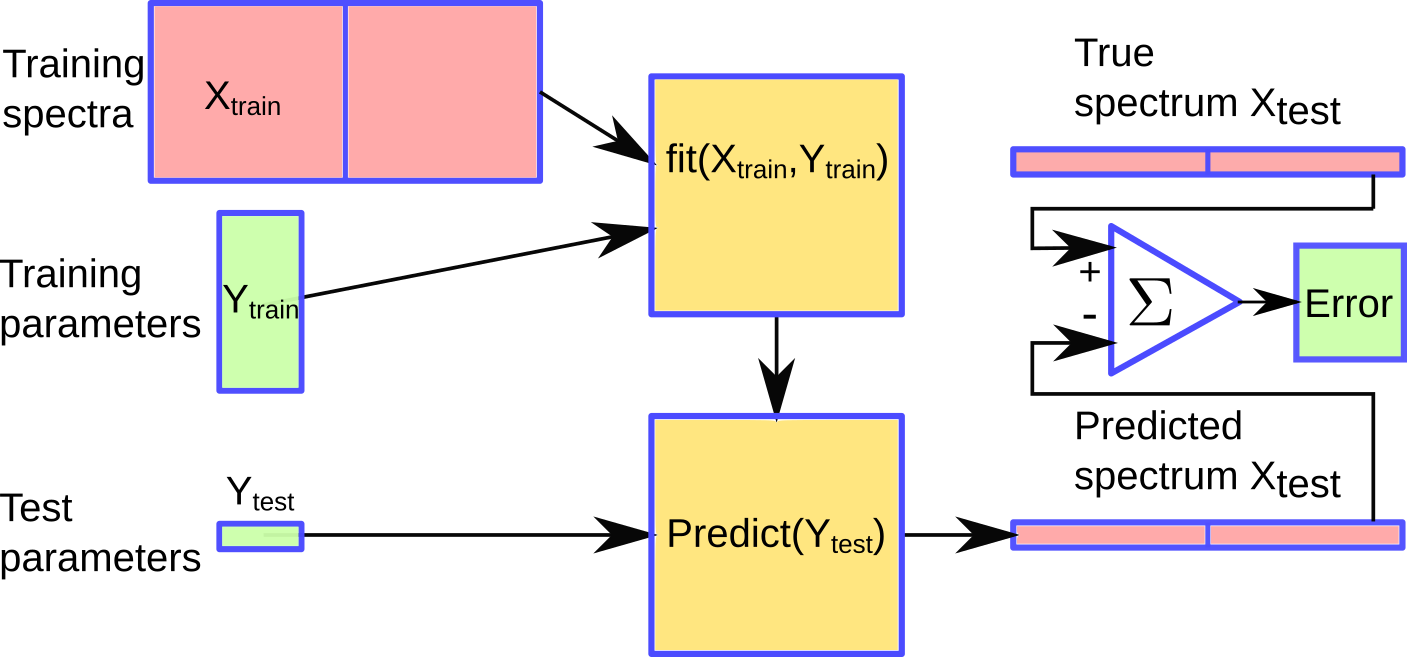
\includegraphics[width=15cm]{./img/MLvariables2.png} 
	\caption[\protect\input{./img/MLvariables2Short.txt}]{\protect\input{./img/MLvariables2.txt}}%
	\label{fig:MLvariables2}
\end{figure}
The training inputs (the training parameters on figure~\ref{fig:MLvariables2}) and outputs (the training spectra in figure~\ref{fig:MLvariables2}) are analysed together by the machine learning algorithm to determine a relationship between the two sets of data. This allows the learning algorithm to predict outputs (predicted spectrum in figure~\ref{fig:MLvariables2}) from new inputs (test parameters in figure~\ref{fig:MLvariables2}). Furthermore, if the new input has a known output, then this can be directly compared with the predicted output to determine how successful supervised learning has been. \par
Unsupervised learning takes the training data and transforms it in some way, without any comparison to any input parameters. Principal component analysis (PCA) is an example of unsupervised learning algorithm, in this application the PCA algorithm takes the Fourier spectrum and encodes each spectra onto a point in PCA space (see section~\ref{sec:PCA} for details)



\subsection{Over fitting}
Over fitting of a machine learning algorithm can be an issue that results from a predicted model that matches the test set too well. This is an issue because most test data has noise variations in the signals and the learning algorithm has learnt these unwanted noise signals, resulting in faulty predictions when new test data is applied. 
\begin{figure}[H]
	\centering
	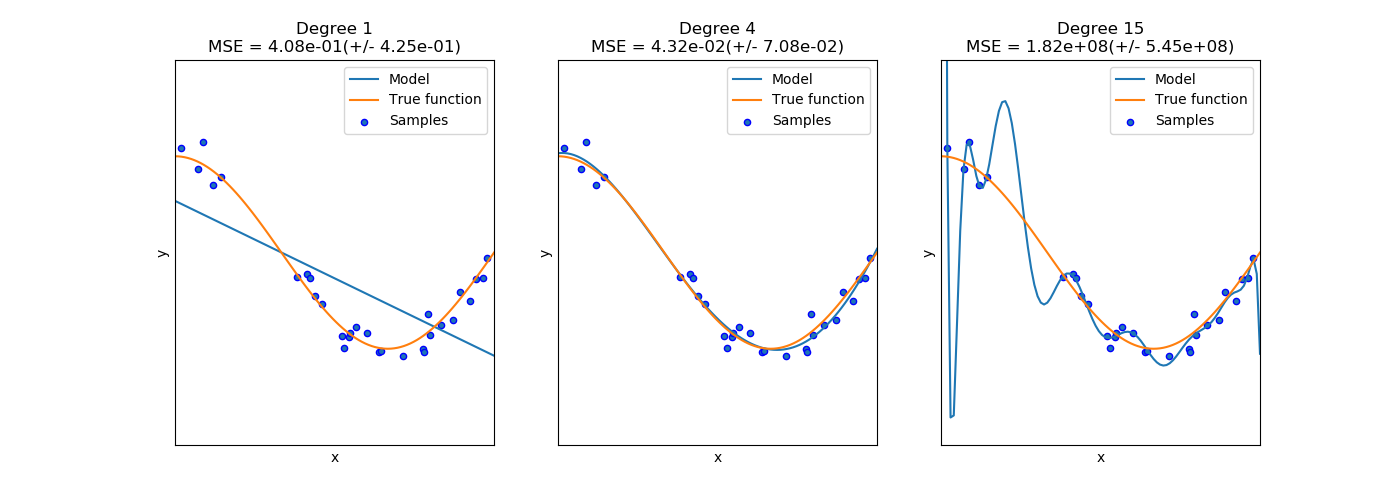
\includegraphics[width=15cm]{./img/Overfitting.png} 
	\caption[\protect\input{./img/OverfittingShort.txt}]{\protect\input{./img/Overfitting.txt}}%
	\label{fig:Overfitting}
\end{figure}

\subsection{Cross-validation}
\label{sec:CrossValidation}
Cross-validation is a process where the data under test is excluded from the training set. This is performed to properly test the ability of a particular model to predict known outcomes. Different types of cross-validation systems are used, two of these are of particular interest in this project: leave one out cross-validation (LOOCV) and holdout cross-validation. Holdout cross-validation is a simple process where a percentage of the data is allocated to the training set, and the remainder is allocated to the test set. Holdout cross-validation was not an option for this project, as we had only 25 valid waveforms. \par
To perform leave one out cross-validation remove one item from the training set and test on this item to predict the outcome and measure the performance, then repeat the process for the next item, until all items have been used as test objects. The performance of the model is based on the average error value for all tests. 
We did perform LOOCV with The Cannon 2 waveforms (section~\ref{sec:TheCannonLOOCV})

\subsection{Comparison metric}
\label{sec:SNRresidual}
Using equation~\ref{eq:SNRhSh} by comparing the original strain $h_{\mathrm{original}}$ to the inferred strain $h_{\mathrm{inferred}}$ gives:
\begin{align}
	\Delta = & \rho_{\mathrm{original}} - \rho_{\mathrm{inferred}}\notag\\
	 = & \dfrac{\left<h_{\mathrm{original}},h_{\mathrm{inferred}}\right>}{\sqrt{\left<h_{\mathrm{original}},h_{\mathrm{original}}\right>}}
	 -\dfrac{\left<h_{\mathrm{original}},h_{\mathrm{inferred}}\right>}{\sqrt{\left<h_{\mathrm{original}},h_{\mathrm{original}}\right>}}\notag\\
	= & \dfrac{\left<h_{\mathrm{original}}-h_{\mathrm{inferred}},h_{\mathrm{original}}\right>}
			{\sqrt{\left<h_{\mathrm{original}},h_{\mathrm{original}}\right>}}\label{eq:DeltaResidual}
\end{align}
Which is an indication of whether it is possible to detect the difference between the original signal and the inferred signal. An alternative metric involves looking directly at the difference between the two signals and seeing if this deviation, $\varepsilon$, is observable:
\begin{align}
\varepsilon=&h_{\mathrm{original}}- h_{\mathrm{inferred}}\\
\rho_\varepsilon = & \dfrac{\left<\varepsilon,\varepsilon\right>}{\sqrt{\left<\varepsilon,\varepsilon\right>}}
				=\sqrt{\left<\varepsilon,\varepsilon\right>}\label{eq:SNRresidual}
\end{align}
For the purpose of this project, we decided to use equation~\ref{eq:SNRresidual} for a comparison metric which is equivalent to the optimal SNR (equation~\ref{eq:SNRopt}) of the residual signal, $\varepsilon$, and therefore we designate this quantity as the residual SNR henceforth.
\subsubsection{Frequency dependent metrics}
In some of the plots in The Cannon (section~\ref{sec:TheCannon}) a frequency dependent metric was used to help determine which frequency values contribute the most towards the residual SNR. To do this, equation~\ref{eq:SNRhSh} was de-constructed as follows:
\begin{equation}
	\zeta(h,f)=\dfrac{\|\tilde{h}(f)\|\sqrt{f}}{A_h(f)},
	\label{eq:zetah}
\end{equation}
where $A_h(f)=\sqrt{S_h(f)}$ is the amplitude spectral density of the advanced LIGO noise curve and $\zeta(h,f)$ is the relative importance of the signal $\tilde{h}(f)$ at frequency $f$. Any errors in the reconstructed signal that occur when $\zeta(h,f)$ is around one or more will contribute significantly to the residual SNR. This metric can also be used to measure complex differences in signals by calculating $\zeta(h_1-h_2)$ as follows:
\begin{equation}
	\zeta(\Delta h,f)=\zeta(h_1-h_2,f)=\dfrac{\|\tilde{h}_1(f)-\tilde{h}_2(f)\|\sqrt{f}}{A_h(f)},
	\label{eq:zetadeltah}
\end{equation}
where $\tilde{h}_1$ and $\tilde{h}_2$ are the two signal to be compared. Values of $\zeta(h_1-h_2,f)$ larger than one indicate parts of the signal where $\tilde{h}_1$ and $\tilde{h}_2$ deviate significantly, leading to a large value of the residual SNR.
\subsection{Principal components analysis}
\label{sec:PCA}
Principal component analysis (PCA) is an example of an unsupervised learning algorithm, that decomposes a matrix $X$ to an ordered set of eigenvectors $v_i$ that form an orthonormal basis for $X$ \cite[eg][]{Clark2015,Wall2003}:
\begin{equation}
	X = \displaystyle\sum_k \beta_k \vec{v}_k
	\label{eq:XpcaExpansion}
\end{equation}
Each eigenvector is called a principal component and the first principal component has the greatest contribution to $X$ and subsequent principal components have equal or less contributions. The ordering of the PCA principal components can be visualised in figure~\ref{fig:PCArelativeimportance}
\begin{figure}[H]
	\centering
	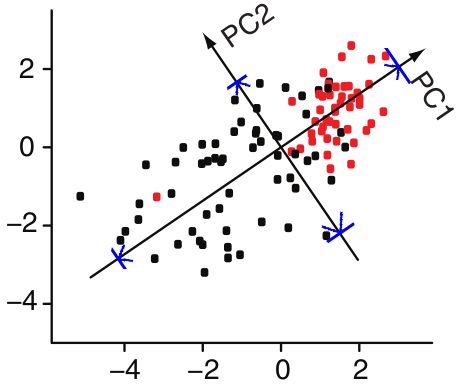
\includegraphics[width=10cm]{./img/PCArelativeimportance.png} 
	\caption[\protect\input{./img/PCArelativeimportanceShort.txt}]{\protect\input{./img/PCArelativeimportance.txt}}%
	\label{fig:PCArelativeimportance}
\end{figure}
The PCA algorithm was implemented with Scikit Learn \cite{scikit-learn} in python. A simplified example of the PCA code is shown here:
\begin{lstlisting}[basicstyle=\small]
pca=PCA(num_components=3)
pca.fit(Xtrain)
PCAspace=pca.transform(Xtrain)
\end{lstlisting}
The first command determines the number of dimensions required for the PCA analysis, we used three dimensions and hence three principal components. The second line trains the PCA algorithm on the training data, and the last line determines the projections onto the three dimensional space, the $\beta$ values from equation~\ref{eq:XpcaExpansion}. Each each row of Xtrain corresponds to a spectrum for a particular EOS, mass ratio, and mean mass. For each of these rows there are three $\beta$ values $\left\lbrace \beta_1, \beta_2, \beta_3 \right\rbrace $ that position that particular spectrum in the PCA space and this is what is plotted in sections~\ref{sec:PCAresults}. 
\subsection{Preprocessing of data}
The gravitation-wave strain data was read from the data supplied and redimensionalised and scaled 50Mpc distance. The data was then converted to the frequency domain using the NFFT function in the Monash GWTools package and saved as a text file for later retrieval, with one column for the time value and the other two columns for the h$_+$ and h$_\times$ respectively. 
\subsection{The Cannon 2 setup}
\label{sec:TheCannonSetup}
The first machine learning algorithm that was used in this project was The Cannon 2 developed by \cite{Casey2016} which was developed to fit stellar spectra to determine information about chemical abundance and uses a modified form of L1 regularisation to predict outcomes. 
\subsubsection{Implementation}
The Cannon 2 training method was performed on the unscaled frequency spectra from the supplied time series data with the frequency values restricted to between 10Hz and 6000Hz.  The low frequency cut-off eliminated the zero frequency from the data, and the high frequency cut-off eliminated signals which were out of the detection band for LIGO.  Furthermore, the spectra of the signals was quite small beyond these frequency cut-off points.  The training set  (X$_{train}$ in figure~\ref{fig:MLvariables2}) consisted of a matrix of the all the spectra. The Cannon algorithm was trained on the following four parameters, chosen to represent major properties of the progenitor neutron stars: the mean mass $\bar{M}$, the compactness $C$, the TOV mass $M_{TOV}$ and the tidal deformation term $\kappa^T_2$. The j-th row of the matrix Y$_{train}$ (figure~\ref{fig:MLvariables2}) consists of the parameters $\left\lbrace \bar{M}, C, M_{TOV}, \kappa^T_2 \right\rbrace$ corresponding to the j-th EOS, mass combination. The j-th row of X$_{train}$ consists of the spectra for the j-th EOS / mass combination.  A simplified version of the Cannon 2 prediction code is shown here:
\begin{lstlisting}[basicstyle=\small]
model=CannonModel(Ytrain,Xtrain,Variances,Parameters) 
model.train()
Xprediction = model(Ytest)
CalcResidualSNR(Xtest,Xprediction)
\end{lstlisting}
This pseudo-code performs the same function as shown in figure~\ref{fig:MLvariables2}. The first two lines perform the fit command, the third line performs the predictive step, and the last line calculates the residual SNR value according to equation~\ref{eq:SNRresidual}. 
 
\subsection{Random forest}
\label{RFsetup}
Random forest is a machine learning algorithm that consists of a large number of individual decision trees. Each decision tree uses a set of inputs chosen from a random subset of all available input parameters, and, from this subset, selects the input of greatest influence as the decision making input. Random forest algorithms have: good accuracy, are tolerant of noise and outliers, are faster than boosting or bagging, and are simple to implement and easy to perform in parallel \cite{Breiman2001}. The random forest algorithm can be used for both regression and classification tasks. For this project we used the random forest regressor available in Scikit Learn package\cite{scikit-learn} to develop our code. We chose to use frequency bin shifting to align spectral features in the real and imaginary domain of the spectrum independently. Simplified pseudo-code without cross-validation is shown here:
\begin{lstlisting}[basicstyle=\small]
alignedXtrain=AlignSprectra(Xtrain,fpeak)
model=RandomForestRegressor()
model.fit(Ytrain, alignedXtrain)
alignedXprediction=model.predict(Ytest)
Xprediction=ReverseAlignment(alignedXprediction,ftest)
CalcResidualSNR(Xtest,Xprediction)
\end{lstlisting}
This code performs the same function as figure~\ref{fig:MLvariables2} with additional steps inserted for the frequency bin shifting.
To implement cross-validation the following modified pseodocode is required:
\begin{lstlisting}[basicstyle=\small]
alignedXtrain=AlignSprectra(Xtrain,fpeak)
model=RandomForestRegressor()
modelfreq=RandomForestRegressor()
model.fit(Ytrain, alignedXtrain)
modelfreq.fit(Ytrain, fpeak) *****
alignedXprediction=model.predict(Ytest)
ftestprediction=modelfreq.predict(Ytest) *****
Xprediction=ReverseAlignment(alignedXprediction,ftestpredict) *****
CalcResidualSNR(Xtest,Xprediction)
\end{lstlisting}
The lines marked with asterix indicate changes required to implement cross-validation. This is required because the learning algorithm does not know how to undo the initial frequency shift.

\subsection{Waveform preparation}
The waveforms that were used for this project were supplied by Luciano Rezzolla from \cite*{Takami2015}. The $h_{22}$ component of the waveform was extracted from the simulation at a distance of 500M$_\odot$. The quantities supplied in these simulation data files were: time (in units of M$_\odot$), $r h_+$, and $r h_\times$ (both in units of M$_\odot$). The distance from the source, $d$, in this project was chosen to be 50Mpc. These values were redimensionalised as:
\begin{align}
& t(\text{s})  =\dfrac{\text{M}_\odot \text{G}}{c^3}t(\text{M}_\odot)\\
& h_{+,d}\left(\text{M}_\odot \right)  =\left(\dfrac{r}{d}\right)h_{+,r} = \dfrac{rh_{+,r}}{d}=\dfrac{rh_{+,r}\left(\text{M}_\odot \right)}{d}\notag \\ 
& h_{+,d}\left(\text{m.m}^{-1}\right)   =\left( rh_{+,r}\left(\text{M}_\odot \right)\right)\times \dfrac{\text{M}_\odot \text{G}}{50 c^2\left[ \text{1 Mpc} \right]}\approx 9.5708\times10^{-22}\left( rh_{+,r}\left(\text{M}_\odot \right)\right),
\end{align}
where $h_{+,r}$ and $h_{+,d}$ are the plus polarisation of the gravitational-wave strain at respective  distances of $r$ and $d$ from the source respectively. The gravitational strain, $h_{+,d}$, is a dimensionless term after redimensionalising. During this thesis $h_{+}$ will refer to $h_{+,d}$, the strain at distance $d=50$Mpc from the source. The time series data was not directly used for this project, this data was converted into the frequency domain by performing a fast Fourier transform on the time series data. As mentioned in section~\ref{sec:NR}, the zero time point coincides with the time of merger and in the following sections, the time series waveforms were truncated to positive time values corresponding to the post-merger region. This simplified the coding process required for frequency scaling (see section~\ref{sec:PCAScaled}) and allowed concentration of the spectral properties of the post-merger spectra. This restriction will be dropped for future investigation into this topic, as we ultimately require a system that works with both the inspiral and post-merger signals.\par
\subsection{Numerical relativity waveforms}

Tables~\ref{tbl:Waveforms1Table}~and~\ref{tbl:Waveforms2Table} show a list of the names of the waveforms available and their corresponding parameters. 

The waveforms designated as GAM2 were simple polytropes with a fixed $\Gamma=2.0$. The spectra generated by these waveforms was qualitatively quite different to the more realistic waveforms with piecewise polytropes (see section~\ref{sec:NR} and table~\ref{tbl:EOSpoly}) and were therefore excluded from the waveforms under test. Furthermore, as we only had two waveforms with an unequal mass ratio, we decided to exclude these waveforms from The Cannon 2 machine learning data set, though these waveforms were still used for PCA decomposition and the random forest analysis.
